\chapter{Elettroni interagenti}

%%%%%%%%%%%%%%%%%%%%%%%
%%%%%% Lezione 1 %%%%%%
%%%%%%%%%%%%%%%%%%%%%%%

\lecture{1}{04/10/2021}

\section{Modello di Hartree}

Il \textbf{modello di Hartree} si preoccupa di andare a descrivere i sistemi che prevedono un'interazione tra elettroni nel medesimo sistema (ad esempio atomi). Prima di addentrarci nella trattazione del modello stesso, facciamo una breve digressione sul concetto di \textbf{particelle identiche}.

\begin{definition}{Particelle identiche}
    Nel momento in cui si considera un sistema, al cui interno sono presenti delle particelle identiche, a seconda del tipo di quest'ultime si deve soddisfare una determinata proprietà di simmetria rispetto allo scambio tra particelle.
\end{definition}

\noindent Identifichiamo con $\psi$ la funzione d'onda di un sistema di particelle. In particolar modo essa sarà $\psi(\overline{x}_1, s_1, \dots, \overline{x}_n, s_n)$, dove $\overline x_i$ e $s_i=\pm \frac 12$ sono rispettivamente la variabile spaziale e la proiezione dello spin lungo l'asse $z$. A questo punto, ricordiamo che possiamo classificare le particelle nel seguente modo:
\begin{itemize}
    \item \textbf{Fermioni}: particelle a spin semi-intero con $\psi$ antisimmetrica rispetto allo scambio tra particelle e seguono la statistica di Fermi - Dirac;
    \item \textbf{Bosoni}: particelle a spin intero o nullo con $\psi$ simmetrica rispetto allo scambio tra particelle e seguono la statistica di Bose - Einstein.
\end{itemize}

\noindent Osserviamo quindi che una funzione d'onda ha queste proprietà di simmetria rispetto lo scambio. La $\hat H$ di un sistema è sempre simmetrica rispetto allo scambio tra particelle, essa è definita, nel modo più generale possibile come:

\begin{equation*}
    \hat H = \sum_{i=1}^N \hat h_i + \hat U_{\text{int}}
\end{equation*}

\noindent dove:
\begin{itemize}
    \item $\hat h_i=\frac{{\hat{\overline{p}}}_i^2}{2m}+\hat V_{\text ext}(\hat{\overline{x}}_i)$ è l'hamiltoniana della particella i-esima e ne indichiamo la sua somma con:
    \begin{equation*}
        \hat H_0 = \sum_{i=1}^N \hat h_i
    \end{equation*}
    \item $\hat U_{\text{int}}$ è il potenziale di interazione che, nel caso elettrostatico, è: 
    \begin{equation*}
        \hat U_{\text{int}}=\frac 12 \sum_{i \neq j}^N\frac{e_0^2}{4\pi\varepsilon_0|\overline x_i - \overline x_j|}
    \end{equation*}
\end{itemize}

\noindent Se non ci fosse questo termine di interazione sapremmo risolvere il problema, infatti avremmo che $\hat H = \hat H_0$, per cui la soluzione esatta sarà data da:
\begin{equation*}
    \hat H_0\psi = E \psi 
\end{equation*}

\noindent Per componenti
\begin{equation*}
    \hat h u_\alpha(\overline x) = \varepsilon_\alpha u_\alpha(\overline x)
\end{equation*}

\noindent dove $\alpha$ rappresenta un set completo di numeri quantici ($n, l, m, m_s$). Sappiamo quindi costruire una soluzione a $n$ particelle come:
\begin{equation*}
    \Phi(\overline{x}_1, \dots, \overline{x}_n)=u_\alpha(\overline{x}_1)u_\beta(\overline{x}_2)\dots u_\nu(\overline{x}_n)
    \ \ \ \ \ \ \ \ \ \
    E = \varepsilon_\alpha + \dots + \varepsilon_\nu
\end{equation*}
\noindent Scritta in questo modo non soddisfa la condizione riguardante lo scambio tra particelle. $\Phi$ è quindi sì soluzione dell'hamiltoniana $H_0$ (hamiltoniana separabile), ma non rispetta la simmetria rispetto lo scambio tra particelle.

\noindent Introduciamo il \textbf{determinante di Slater} distinguendo il caso \textbf{fermionico} da quello \textbf{bosonico}.

\subsection{Determinante di Slater per fermioni}
\noindent Affinché soddisfi questa richiesta, costruiamo il \textbf{determinante di Slater}. Partendo dalla scelta di $\alpha \dots \nu$ possiamo costruire una funzione d'onda che è una combinazione lineare in cui si permutano gli indici. La matrice si costruisce mantenendo $u_i$ costante sulle righe e variando la particella in considerazione e mantenendo la particella costante sulle colonne e variando la $u_i$.
\begin{equation*}
    \text{Determinante di Slater }=
    \frac{1}{\sqrt{N!}}
    \begin{vmatrix}
        u_\alpha(1) & u_\alpha(2) & \cdots & u_\alpha(N) \\
        u_\beta(1) & u_\beta(2) & \cdots & u_\beta(N) \\
        \vdots & \vdots & \ddots & \vdots \\
        u_\nu(1) & u_\nu(2) & \cdots & u_\nu(N) \\
    \end{vmatrix}
\end{equation*}
Osserviamo che questo è il determinante di una matrice e corrisponde alla somma di $N!$ addendi, si tratta di diverse permutazioni con diversi segni (a causa del calcolo del determinante). Sono tutti addendi a cui corrispondono funzioni d'onda ortogonali tra loro. Se sono tutti ortogonali posso facilmente normalizzare la funzione d'onda complessiva con un termine $\frac{1}{\sqrt{N!}}$. Concludiamo quindi che questa funzione d'onda soddisfa le proprietà di simmetria rispetto lo scambio. Questo lo notiamo soprattutto nello scambio tra colonne, per cui, uno scambio tra esse produce un segno meno.

Ricordiamo che il determinante di una generica matrice è diverso da zero se tutte le righe e colonne sono \textit{linearmente indipendenti}. Questo significa che se tentassimo di costruire un sistema di N particelle con 2 particelle aventi lo stesso set di numeri quantistici, il determinante si annulla, per cui non posso costruire il determinante di Slater. Questo risultato permette di enunciare il seguente principio.

\begin{definition}{Principio di esclusione di Pauli}
    In un sistema di particelle identiche, soluzioni dell'hamiltoniana $\hat H$, non posso costruire una $\psi$ che abbia al suo interno funzioni d'onda con lo stesso set di numeri quantici.
\end{definition}

\subsection{Determinante di Slater per bosoni}
Se abbiamo un sistema bosonico, la nostra funzione complessiva sarà simmetrica rispetto lo scambio tra particelle. Osserviamo che vi è un modo semplice per costruire un sistema di funzioni d'onda che soddisfi questa simmetria. Partendo anzitutto dagli stati a particella singola si costruisce il determinante di Slater, tuttavia, a differenza del caso fermionico, ogni segno negativo è trasformato in positivo. Vediamo quindi che non vi è più il problema della \textit{linearità indipendente} di righe e colonne. Quindi, nel caso di bosoni, posso costruire una funzione a N particelle con lo stesso set di numeri quantici, non avrò quindi alcuni equivalente del principio di esclusione di Pauli per i bosoni.

Questo però comporta delle complicazioni in termini del fattore di normalizzazione. Se abbiamo N bosoni che occupano stati a singola particella diversa, abbiamo sempre una normalizzazione pari a $\frac{1}{\sqrt{N!}}$.

Possiamo però ora mettere più di una particella con lo stesso $\alpha$ nello stesso stato, non è detto che siano ortonormali tra loro, per cui il coefficiente di normalizzazione non è più $\frac{1}{\sqrt{N!}}$. Supponiamo di mettere un certo numero di particelle nello stato $n_\alpha$, avremo allora questo coefficiente di normalizzazione:

\begin{equation*}
    \frac{1}{\sqrt{N!\Pi_\alpha n_\alpha!}}
\end{equation*}

Abbiamo quindi, sia nel caso fermionico che bosonico, queste funzioni d'onda che sono delle soluzioni esatte della hamiltoniana separabile:
\begin{equation*}
    \hat H_0 = \sum_{i=1}^N \hat h_i
\end{equation*}
Le funzioni d'onda formano anche una base per lo spazio di Hilbert. Quindi sono un sistema di autostati per $\hat H_0$ e si può pensare di sviluppare su questa base nel momento in cui si ha anche delle interazioni del tipo:
\begin{equation*}
    \hat H = \hat H_0 + \hat U_{\text{int}}
\end{equation*}
Lo spazio che quindi ho costruito con questa base, lo possiamo usare per lavorare anche il caso di particelle interagenti.

Il modello più semplice per descrivere l'interazione elettrone-elettrone è il \textbf{modello di Hartree}, consiste nello scrivere l'equazione agli autovalori a particella singola a cui però si somma un termine che descrive l'interazione con gli altri elettroni noto come \textbf{potenziale di Hartree}. L'equazione agli autovalori risulta quindi:

\begin{equation*}
    \bigg[-\frac{\hbar^2}{2m}\nabla^2 + V_{\text{ext}}(\overline x) + V_H(\overline x)\bigg]u_\alpha=\varepsilon_\alpha u_\alpha
\end{equation*}
Nel caso elettrostatico $V_H(\overline x)$ è:
\begin{equation*}
    V_H(\overline x) = \frac{e_0^2}{4\pi\varepsilon_0}\int d^3\overline{x}' \frac{n(\overline{x}')}{|\overline x - \overline{x}'|}
\end{equation*}
dove $n(\overline{x}')=\sum_i^N|u_i(\overline{x}')|^2$ è la densità di carica associata a tutti gli elettroni e gli $u_i(\overline x)$ sono gli autostati dell'hamiltoniana $\hat H_0$.

In questo caso stiamo facendo un'approssimazione di campo medio, tuttavia in questa relazione stiamo considerando anche un termine di autointerazione che va, ovviamente, risolto.

Il modello di Hartree risolve il problema attraverso una soluzione autoconsistente. Si procede attraverso una procedura iterativa, per cui:
\\
\textbf{Ciclo 0:}
\begin{itemize}
    \item Si trascura il termine $V_H$, si risolve l'equazione agli autovalori e si trovano gli stati $u_i^0$;
    \item Si parte dagli orbitali a energia più bassa e si riempiono i vari orbitali;
    \item Con questi stati $u_i^0$ si costruisce la $n^0(\overline{x})$;
    \item Nota $n^0(\overline{x})$ ricavo $V_H(\overline x)^0$.
\end{itemize}
\textbf{Ciclo 1:}
\begin{itemize}
    \item Inserisco nell'equazione il termine $V_H^0$, si risolve l'equazione agli autovalori e si trovano gli stati $u_i^1$;
    \item Si parte dagli orbitali a energia più bassa e si riempiono i vari orbitali;
    \item Con questi stati $u_i^1$ si costruisce la $n^1(\overline{x})$;
    \item Nota $n^1(\overline{x})$ ricavo $V_H^1(\overline x)$.
\end{itemize}
\textbf{Ciclo j:}
\begin{itemize}
    \item Inserisco nell'equazione il termine $V_H^{j-1}$, si risolve l'equazione agli autovalori e si trovano gli stati $u_i^j$;
    \item Si parte dagli orbitali a energia più bassa e si riempiono i vari orbitali;
    \item Con questi stati $u_i^j$ si costruisce la $n^j(\overline{x})$;
    \item Nota $n^j(\overline{x})$ ricavo $V_H^j(\overline x)$.
\end{itemize}
Itero questo procedimento finché non raggiungo un risultato consistente tale per cui le funzioni d'onda N-1 e N differiscono di poco tra loro. Tramite questo processo raggiungo una soluzione autoconsistente.
Per quanto riguarda invece l'energia totale, essa non sarà data da:
\begin{equation*}
    E=\sum_i\varepsilon_i=\sum_i\bra{u_i}\hat h + V_H\ket{u_i}=\sum_i \bra{u_i}\hat h\ket{u_i}+\int d^3x V_h(\overline x)|u_i(\overline x)|^2
\end{equation*}
Analizziamo bene l'ultimo integrale:
\begin{equation*}
    \frac{e_0^2}{4\pi\varepsilon_0}\int d^3 \overline x'\int d^3 \overline x \frac{n(\overline x)n(\overline{x}')}{|\overline x - \overline{x}'|}
\end{equation*}
Stiamo contando due volte l'interazione coulombiana, quindi a questo risultato si pone davanti un fattore $\frac 12$. Quindi l'energia sarà:
\begin{equation*}
    E=\sum_i\varepsilon_i - \frac 12 \frac{e_0^2}{4\pi\varepsilon_0}\int d^3 \overline x'\int d^3 \overline x \frac{n(\overline x)n(\overline{x}')}{|\overline x - \overline{x}'|} = \sum_i\varepsilon_i - E_H
\end{equation*}
Questo modello è molto semplice, ci permette di descrivere in particolare il caso di 2 elettroni in interazione come nell'atomo di elio. Precisiamo però che nello stato fondamentale funziona, però già nello stato eccitato vi è una complicazione.
\subsection*{Atomo di He}
Ripartiamo dall'hamiltoniana del sistema:
\begin{equation*}
    \hat H = \hat h_1 + \hat h_2 + \frac{e_0^2}{4\pi\varepsilon_0 |\overline{x}_1-\overline{x}_2|} \text{   dove   } \hat h = -\frac{\hbar^2}{2m}\nabla^2-\frac{e_0^2 Z}{4\pi\varepsilon_0 r}
\end{equation*}
La ricerca di soluzioni approssimate ci ha portati all'utilizzo della teoria perturbativa considerando l'interazione come una perturbazione. Per l'hamiltoniana di singola particella abbiamo:
\begin{equation*}
    \hat h u_{nlmm_s}(\overline x)=\varepsilon_nu_{nlmm_s}(\overline x)
\end{equation*}
Se abbiamo, in questo caso, due particelle bisogna decidere quali stati occupare: $1s^2$ oppure $1s2s$. Siccome siamo interessati allo stato eccitato, consideriamo quest'ultima. Bisogna ora scegliere come costruire il determinante di Slater.

Vi sono quattro possibili scelte a seconda di come andiamo a posizionare gli elettroni:

Ogni configurazione è un determinante di Slater e vi sono 4 stati degeneri. Una volta individuata la soluzione esatta, si procede con l'accendere la perturbazione e la si tratta con la teoria delle perturbazioni. Partiamo con il definire il potenziale di interazione

\begin{equation*}
    U_{\text{int}}=\frac{e_0^2}{4\pi\varepsilon_0|\overline{x}_1-\overline{x}_2|}
\end{equation*}

Successivamente dobbiamo costruire la matrice di elementi: $\bra j U_{\text{int}}\ket i$ e per farlo dobbiamo diagonalizzarla sul sottospazio degli stati degeneri. In questo caso risulta opportuno trovare delle simmetrie così da facilitare la risoluzione del problema agli autovalori. In maniera molto intuitiva, gli operatori di spin, commutano con l'hamiltoniana, infatti $\hat{\overline S} = \hat{\overline{S}}_1+\hat{\overline{S}}_2$, da cui possiamo costruire gli operatori $\hat S^2$ ed $\hat S_z$.
Vediamo ora se gli autostati dati dal determinante di Slater sono dei buoni autostati di $\hat H$, $\hat S^2$ ed $\hat S_z^2$:
\begin{equation*}
    \psi^{(1)}=\frac {1}{\sqrt 2} \begin{vmatrix} u_{1s}(1)\alpha(1) & u_{1s}(2)\alpha(2) \\ u_{2s}(1)\alpha(1) & u_{2s}(2)\alpha(2) \end{vmatrix}=\frac {1}{\sqrt 2} \big[u_{1s}(1)u_{2s}(2)\alpha(1)\alpha(2)-u_{1s}(2)u_{2s}(1)\alpha(2)\alpha(1)\big]
\end{equation*}
\begin{equation*}
    \psi^{(1)}=\frac {1}{\sqrt 2}\alpha(1)\alpha(2)\big[u_{1s}(1)u_{2s}(2)-u_{1s}(2)u_{2s}(1)\big]
\end{equation*}
osserviamo che la componente di spin è simmetrica rispetto allo scambio delle due particelle, mentre la componente spaziale è antisimmetrica.
Pertanto dalla funzione $\psi^{(1)}$ abbiamo il primo \textbf{stato di tripletto}: $\ket{11}$, lo stesso ragionamento lo possiamo applicare per $\psi^{(2)}$ dove in questo caso abbiamo $\beta(1)\beta(2)$, cioè il secondo \textbf{stato di tripletto}: $\ket{1-1}$. Tuttavia se costruissi i determinanti di Slater per $\psi^{(2)}$ e $\psi^{(4)}$, essi non si fattorizzano in una componente spaziale e una di spin, per cui non sono delle buone funzioni/autostati. Se però eseguissimo una combinazione lineare di $\psi^{(2)}$ e $\psi^{(4)}$ troveremmo due stati ortogonali che possono essere fattorizzati in una componente spaziale e una di spin, ottenendo: $\ket{10}$ (terzo \textbf{stato di tripletto}) e $\ket{00}$ \textbf{stato di singoletto}). Quindi avremo tre \textbf{stato di tripletto} simmetrici e uno \textbf{stato di singoletto} antisimmetrico rispetto allo scambio tra le due particelle.

Quindi se scelgo ora questa nuova base $\psi^{(1)}$, $\psi^{(2)}$, $\psi^{(3')}$ e $\psi^{(4')}$, ho che la perturbazione è già diagonale ed è indipendente dallo spin. Per cui non resta che valutare, rispettivamente per il tripletto e il singoletto queste quantità:
\begin{equation*}
    \bra{\psi_T}\frac{e_0^2}{4\pi\varepsilon_0|\overline{x}_1-\overline{x}_2|}\ket{\psi_T} = J - K
\end{equation*}
\begin{equation*}
    \bra{\psi_S}\frac{e_0^2}{4\pi\varepsilon_0|\overline{x}_1-\overline{x}_2|}\ket{\psi_S} = J + K
\end{equation*}
Queste due quantità vengono chiamate rispettivamente:
\begin{equation*}
    \text{Integrale diretto } J = \frac{e_0^2}{4\pi\varepsilon_0}\int d^3x d^3x'u_{1s}^*(\overline x)u_{1s}(\overline x)u_{2s}^*(\overline{x}')u_{2s}(\overline{x}')\frac{1}{|\overline x - \overline{x}'|}
\end{equation*}
\begin{equation*}
    \text{Integrale di scambio } K = \frac{e_0^2}{4\pi\varepsilon_0}\int d^3x d^3x'u_{1s}^*(\overline x)u_{1s}(\overline{x}')u_{2s}^*(\overline{x}')u_{2s}(\overline{x})\frac{1}{|\overline x - \overline{x}'|}
\end{equation*}
In questo caso possiamo osservare che il contributo dell'interazione sarà minore nel caso del tripletto rispetto a quello del singoletto. Inoltre $K$ è un effetto puramente quantistico, non ha alcun analogo classico.
Pertanto per l'atomo di elio, $J\approx 9.2 \text{ eV}$, mentre $K \approx 0.8 \text{ eV}$. In questo caso però l'\textbf{integrale di scambio} non c'è nel \textbf{modello di Hartree}, lo abbiamo trovato in regime perturbativo, ma non possiamo usare la teoria delle perturbazioni per gli atomi più grandi, a più elettroni. Le funzioni d'onda idrogenoidi non sono un buon punto di partenza, bisogna introdurre qualcosa che tenga conto di $K$ e questo viene fatto dal seguente modello.

\section{Modello di Hartree-Fock}

%%%%%%%%%%%%%%%%%%%%%%%
%%%%%% Lezione 2 %%%%%%
%%%%%%%%%%%%%%%%%%%%%%%

\lecture{2}{08/10/2021}
Abbiamo visto che il \textbf{modello di Hartree} non tiene conto di questo termine di scambio che abbiamo identificato con $K$. Quest'ultimo però compare nella teoria delle perturbazione e lo abbiamo visto quando abbiamo trattato l'eccitazione dell'atomo di He. Necessitiamo dunque di un nuovo modello che tenga in considerazione $K$. Consideriamo l'hamiltoniana dell'interazione degli elettroni di He:
\begin{equation*}
    \hat H = \frac12\frac{e_0^2}{4\pi\varepsilon_0}\sum_{i\neq j}\frac{1}{|\overline{x}_i-\overline{x}_j|}-\frac 12\sum_{i}V_H(\overline{x}_i)
\end{equation*}
\noindent dove $V_H$ è il potenziale introdotto per descrivere l'interazione degli elettroni ed è un potenziale sferico.
Nel \textbf{modello di Hartree-Fock}, si fa la seguente approssimazione: la funzione di stato fondamentale del sistema a multielettroni è definita da un singolo determinante di Slater:
\begin{equation*}
    \psi(\{x_i\})=\underbrace{\frac{1}{\sqrt{N!}}}_{\text{norm.}}\underbrace{\sum_{p}}_{\text{perm.}}(-1)^p\hat p \underbrace{u_\alpha(1)u_\beta(2)\dots u_\nu(N)}_{\Phi}
\end{equation*}
\noindent Questa è l'assunzione che si fa, ma non sappiamo quale $\Phi$ scegliere. Abbiamo l'hamiltoniana esatta $\hat H$ e possiamo calcolare l'energia media dell'hamiltoniana con la funzione d'onda $\psi$ dell'approssimazione:
\begin{equation*}
    \bra\psi \hat H\ket\psi=E
\end{equation*}
Come scegliamo quindi $\Phi$ in maniera da minimizzare l'energia $E$? Si tratta di un problema già trattato con il principio variazionale, in particolar modo è molto simile al caso del ground-state dell'atomo di elio, in cui siamo partiti da una particolare $\psi$.\\
Nel \textbf{modello di Hartree-Fock} invece non facciamo alcuna assunzione sulla funzione d'onda $\psi$, noi vogliamo minimizzare l'energia. In questo caso l'energia è un funzionale delle funzioni d'onda $\{u_\alpha\}$, che indichiamo così:
\begin{equation*}
    E\big[u_\alpha\{x_i\}\big]
\end{equation*}
Per poter minimizzare questo funzionale dobbiamo introdurre l'operazione di \textbf{derivata di un funzionale} (vedi Appendice 1).\\
Prima di fare ciò, cerchiamo di dare una forma all'energia:
\begin{equation*}
    \bra\psi \hat H\ket\psi=E\big[u_\alpha\{x_i\}\big]
\end{equation*}
Introduciamo l'\textbf{operatore di antisimmetrizzazione}:
\begin{equation*}
    \hat A = \frac{1}{N!}\sum_p(-1)^p\hat p
\end{equation*}
\noindent Proprietà:
\begin{enumerate}
    \item \textbf{Autoaggiunto}: $\forall\psi,\phi \ \ \ \ip{\psi}{\hat A \phi}=\ip{\hat A \psi}{\phi}$
    \item \textbf{Idempotente}: $\hat A ^2 = \hat A$
\end{enumerate}
Con questa nuova definizione, possiamo riscrivere $\psi$ nel seguente modo:
\begin{equation*}
    \psi = \sqrt{N!}\hat A \Phi
\end{equation*}
Valutiamo gli elementi di matrice di $\hat H$ sulla base $\psi$:
\begin{equation*}
    \hat H = \sum_{i=1}^N \hat h_i + \frac 12 \sum_{i\neq j}^NV_{ij} 
\end{equation*}
\begin{equation*}
    \hat h_i = -\frac{\hbar^2}{2m}\nabla_i^2+V_{\text{ext}}(\overline{x}_i) \ \ \ \ \ \ \ \ \ \ V_{ij}=\frac{e_0^2}{4\pi\varepsilon_0|\overline{x}_i-\overline{x}_j|}
\end{equation*}
Siccome $\hat H$ è \textbf{pari} rispetto allo scambio tra particelle, questo significa che $[\hat A, \hat H]=0$
\begin{equation*}
    \begin{aligned}
        \bra\psi \hat H\ket\psi
        & =\bra{\sqrt{N!}\hat A \Phi}\hat H\ket{\sqrt{N!}\hat A \Phi} \\
        & =N!\bra{\Phi} \hat A \hat H \hat A \ket{\Phi} \text{ usiamo che }[\hat A, \hat H]=\hat A\hat H - \hat H \hat A = 0\\
        & =N!\bra{\Phi} \hat H \hat A \hat A \ket{\Phi} \\
        & =N!\bra\Phi\hat H \hat A^2 \ket\Phi \text{ proprietà 2 di }\hat A\\
        & =N!\bra\Phi\hat H\hat A\ket\Phi \\
        & = E
    \end{aligned}
\end{equation*}
Valutiamo ciascun contributo separatamente:
\begin{equation*}
    \hat H = \sum_{i=1}^N \hat h_i + \frac 12 \sum_{i\neq j}^NV_{ij} 
\end{equation*}
Prendiamo $i=1$ e scriviamo $\Phi$ in maniera esplicita:
\begin{equation*}
    \begin{aligned}
        N!\mel{\Phi}{\hat h_1\hat A}{\Phi}
        & = N!\mel{u_\alpha(1)\dots u_\nu(N)}{\hat h_1}{\hat A u_\alpha(1)\dots u_\nu(N)} \\
        & = N!\mel{u_\alpha(1)\dots u_\nu(N)}{\hat h_1}{\frac{1}{N!} u_\alpha(1)\dots u_\nu(N)}  \ \hat h_1 \text{ agisce su part. 1}\\
        & = \mel{u_\alpha(1)}{\hat h_1}{u_\alpha(1)}\underbrace{\ip{u_\beta(2)\dots u_\nu(N)}{u_\beta(2)\dots u_\nu(N)}}_{\ip{u_\alpha}{u_\beta}=\delta_{\alpha\beta}}\\
        & = \mel{u_\alpha(1)}{\hat h_1}{u_\alpha(1)} 
    \end{aligned}
\end{equation*}
Questo risultato vale per tutte le $N$ particelle:
\begin{equation*}
    \begin{aligned}
        \mel{u_\alpha(1)}{\hat h_1}{u_\alpha(1)} + \mel{u_\beta(2)}{\hat h_2}{u_\beta(2)} + \dots + \mel{u_\nu(N)}{\hat h_N}{u_\nu(N)} 
        & = \mel{\psi}{\sum_i \hat h_i}{\psi} \\
        & = \sum_\mu\mel{\mu}{\hat h}{\mu}
    \end{aligned}
\end{equation*}
dove la somma è eseguita su $\mu$ che rappresenta tutto il set di numeri quantici del sistema, visto che $\hat h$ è la stessa per tutte le particelle.\\
Consideriamo il termine che descrive le interazioni:
\begin{equation*}
    \begin{aligned}
    \mel{\psi}{\frac12\sum_{i\neq j}^N V_{ij}}{\psi}
    & =\mel{\sqrt{N!}\hat A \Phi}{\frac12\sum_{i\neq j}^N V_{ij}}{\sqrt{N!}\hat A \Phi} \\
    & =N!\mel{\hat A \Phi}{\frac12\sum_{i\neq j}^N V_{ij}}{\hat A \Phi} \\
    & =N!\mel{\Phi}{\frac12\sum_{i\neq j}^N V_{ij}\hat A^2}{\Phi} \\
    & =N!\mel{\Phi}{\frac12\sum_{i\neq j}^N V_{ij}\hat A}{\Phi} \\
    \end{aligned}
\end{equation*}
Prendiamo una singola coppia di particelle che interagisce: $i=1$, $j=2$:
\begin{equation*}
    \begin{aligned}
    N!\mel{\Phi}{\frac12 V_{12}\hat A}{\Phi}
    & = N!\mel{u_\alpha(1)u_\beta(2)\dots u_\nu(N)}{\frac12 V_{12}\hat A}{u_\alpha(1)u_\beta(2)\dots u_\nu(N)} \\
    & = \mel{u_\alpha(1)u_\beta(2)}{\frac 12 V_{12}}{u_\alpha(1)u_\beta(2)}-\mel{u_\alpha(1)u_\beta(2)}{\frac 12 V_{12}}{u_\alpha(2)u_\beta(1)}
    \end{aligned}
\end{equation*}
In questo caso abbiamo 2 contributi, perché il secondo contributo deriva dallo scambio delle due particelle:
\begin{equation*}
    \begin{aligned}
    \mel{u_\alpha(1)u_\beta(2)}{\frac 12 V_{12}}{u_\alpha(1)u_\beta(2)}
    & = \frac 12 \int d^3x_1d^3x_2u_\alpha^*(1)u_\beta^*(2)V_{12}u_\alpha(1)u_\beta(2) \\
    & = \frac 12 \mel{\alpha\beta}{V_{12}}{\alpha\beta}
    \end{aligned}
\end{equation*}
\begin{equation*}
    \begin{aligned}
    -\mel{u_\alpha(1)u_\beta(2)}{\frac 12 V_{12}}{u_\alpha(2)u_\beta(1)}
    & = - \frac 12 \int d^3x_1d^3x_2u_\alpha^*(1)u_\beta^*(2)V_{12}u_\beta(1)u_\alpha(2) \\
    & = - \frac 12 \mel{\alpha\beta}{V_{12}}{\beta\alpha}
    \end{aligned}
\end{equation*}
A questo punto per valutare i contributi di tutte le particelle in interazione, fissiamo le particelle e facciamo variare i numeri quantici:
\begin{equation*}
    \mel{\psi}{\frac 12 \sum_{i\neq j}^NV_{ij}}{\psi}=\frac 12 \sum_{\mu\nu}(\underbrace{\mel{\mu\nu}{V_{12}}{\mu\nu}}_{\mathclap{\text{Integrale}\\ \text{diretto}}}-\underbrace{\mel{\mu\nu}{V_{12}}{\nu\mu})}_{\mathclap{\text{Integrale} \\ \text{di scambio}}}=\frac 12 \sum_{\mu\nu}(J_{\mu\nu}-K_{\mu\nu})
\end{equation*}
Pertanto l'energia totale sarà quindi:
\begin{equation*}
    E=\sum_\mu\mel{\mu}{\hat h}{\mu}+\frac 12\sum_{\mu\nu}(J_{\mu\nu}-K_{\mu\nu})
\end{equation*}
Osserviamo che, mentre nel \textbf{modello di Hartree} c'erano dei termini spuri che descrivevano una interazione dell'elettrone con se stesso, nel \textbf{modello di Hartree-Fock} quando poniamo $\mu=\nu$, il termine \textit{diretto} viene eliminato da quello di \textit{scambio}.\\
Ora che abbiamo la forma esplicita dell'energia, dobbiamo miniminizzarne il suo funzionale. Tuttavia non possiamo semplicemente porre che la sua derivata sia nulla, abbiamo una compliazione aggiuntiva perché bisogna rispettare la \textbf{condizione di ortonormalità} $\ip{u_\alpha}{u_\beta}=\delta_{\alpha\beta}$. Consideriamo quindi il problema come un \textbf{problema con i minimi vincolati} e per risolverlo, utilizziamo i \textbf{moltiplicatori di Lagrange} $\lambda$:
\begin{equation*}
    \pderivative{(f(\overline x)-\lambda g(\overline x))}{\overline x}=0
\end{equation*}
dove $f(\overline x)$ è la nostra funzione che vogliamo minimizzare mentre $g(x)$ il nostro vincolo. \\

%%%%%%%%%%%%%%%%%%%%%%%
%%%%%% Lezione 3 %%%%%%
%%%%%%%%%%%%%%%%%%%%%%%

\lecture{3}{11/10/2021}
Nel caso dei funzionali come $E\big[u_\alpha\big]$ con vincolo $\ip{u_\alpha}{u_\beta}-\delta_{\alpha\beta}=0$ utilizziamo $\Lambda_{\alpha\beta}$ come moltiplicatore di Lagrange:
\begin{equation*}
    \functionalderivative{u_\alpha^*(\overline x)}\bigg(E\big[\{u_\alpha\},\{u^*_\alpha\}\big]-\Lambda_{\alpha'\beta'}(\ip{u_{\alpha'}}{u_{\beta'}}-\delta_{\alpha'\beta'})\bigg)=0
\end{equation*}
\textbf{Termine} $\ip{u_{\alpha'}}{u_{\beta'}}$:
\begin{equation*}
    \functionalderivative{u_\alpha^*(\overline x)}\int d^3x'u_{\alpha'}^*(\overline{x}')u_{\beta'}(\overline{x}')=u_{\beta'}(\overline x)
\end{equation*}
\textbf{Termine} $\sum_{\mu}\mel{\mu}{\hat h}{\mu}$:
\begin{equation*}
    \functionalderivative{u_\alpha^*(\overline x)}\int d^3x'u_\mu^*(\overline{x}')\hat h u_\mu(\overline{x}')=\delta_{\alpha\mu}\hat h u_\alpha(\overline x)
\end{equation*}
\textbf{Termine} $\frac 12\sum_{\mu\nu}J_{\mu\nu}$:
\begin{equation*}
    \functionalderivative{u_\alpha^*(\overline x)}\frac 12 \sum_{\mu\nu}\int d^3x' d^3x''u_\mu^*(\overline{x}')u_\nu^*(\overline{x}'')\frac{e_0^2}{4\pi\varepsilon_0|\overline{x}'-\overline{x}''|}u_\mu({\overline{x}'})u_\nu(\overline{x}'')
\end{equation*}
Se $\mu=\alpha \vee \nu=\alpha$ ho due contributi, prendiamo $\mu=\alpha$ e semplifichiamo il fattore $\frac 12$
\begin{equation*}
    \functionalderivative{u_\alpha^*(\overline x)} \sum_{\nu}\int d^3x' u_\alpha^*(\overline{x}')u_\alpha(\overline{x}') \int d^3x''u_\nu^*(\overline{x}'')\frac{e_0^2}{4\pi\varepsilon_0|\overline{x}'-\overline{x}''|}u_\nu(\overline{x}'') =
\end{equation*}
\begin{equation*}
    = \underbrace{\sum_{\nu}\int d^3x''u_\nu^*(\overline{x}'')u_\nu(\overline{x}'')\frac{e_0^2}{4\pi\varepsilon_0|\overline{x}'-\overline{x}''|}}_{\text{Potenziale di Hartree}}u_\alpha(\overline x)=V_{\text{Hartree}}(\overline x)u_\alpha(\overline x)
\end{equation*}
\textbf{Termine} -$\frac 12\sum_{\mu\nu}K_{\mu\nu}$:
\begin{equation*}
    -\functionalderivative{u_\alpha^*(\overline x)}\frac 12 \sum_{\mu\nu}\int d^3x' d^3x''u_\mu^*(\overline{x}')u_\nu^*(\overline{x}'')\frac{e_0^2}{4\pi\varepsilon_0|\overline{x}'-\overline{x}''|}u_\nu({\overline{x}'})u_\mu(\overline{x}'')
\end{equation*}
Come prima, se $\mu=\alpha \vee \nu=\alpha$ ho due contributi, prendiamo $\mu=\alpha$ e semplifichiamo il fattore $\frac 12$
\begin{equation*}
    - \functionalderivative{u_\alpha^*(\overline x)} \sum_{\nu}\int d^3x' u_{\alpha}^*(\overline{x}')\int d^3x''u_\nu^*(\overline{x}')u_\nu(\overline{x}'')\frac{e_0^2}{4\pi\varepsilon_0|\overline{x}'-\overline{x}''|}u_\alpha(\overline{x}') =
\end{equation*}
\begin{equation*}
    = -\sum_\nu \int d^3x''u_\nu^*(\overline{x}'')u_\alpha(\overline{x}'')\frac{e_0^2}{4\pi\varepsilon_0|\overline{x}-\overline{x}''|}u_\nu(\overline{x})=-\hat V_{\text{Fock}}(\overline x)u_\alpha(\overline x)
\end{equation*}
Mettendo insieme tutti i termini abbiamo:
\begin{equation*}
    \hat h(\overline x) u_\alpha(\overline x)+\hat V_H(\overline x)u_\alpha(\overline x)-\hat V_F(\overline x) u_\alpha(\overline x) = \Lambda_{\alpha\beta'}u_{\beta'}(\overline x)
\end{equation*}
Specifichiamo meglio questi contributi:
\begin{itemize}
    \item $J_{\mu\nu}=\mel{\mu\nu}{V_{12}}{\mu\nu}$: senza perdere in generalità, distinguiamo la componente spaziale da quella di spin come: $\mu=\mu\sigma$, $\sigma=\pm\frac 12$, quindi
    \begin{equation*}
        J_{\mu\nu}=\mel{\mu\nu}{V_{12}}{\mu\nu}=\mel{\mu\sigma\nu\sigma'}{V_{12}}{\mu\sigma\nu\sigma'}=\mel{\mu\nu}{V_12}{\mu\nu}\ip{\sigma\sigma'}{\sigma\sigma'}
    \end{equation*}
    dal momento che $V_{12}$ non dipende dallo spin, rimane solo la componente spaziale. Pertanto nel valutare l'energia di Hartree, l'integrale è sì un integrale spaziale, ma la somma viene eseguita anche sullo spin:
    \begin{equation*}
        E_H=\frac 12\sum_{\mu\nu\sigma\sigma'}\mel{\mu\nu}{V_{12}}{\mu\nu}
    \end{equation*}
    \item $K_{\mu\nu}=\mel{\mu\nu}{V_{12}}{\nu\mu}$: stesso discorso vale per l'integrale di scambio, tuttavia, il suo valore è non nullo se gli spin hanno lo stesso verso:
    \begin{equation*}
        K_{\mu\nu}=\mel{\mu\nu}{V_{12}}{\nu\mu}=\mel{\mu\sigma\nu\sigma'}{V_{12}}{\nu\sigma'\mu\sigma}=-\frac 12 \sum_{\mu\nu\sigma}K_{\mu\sigma\nu\sigma}
    \end{equation*}
\end{itemize}
Possiamo fare un passo in più considerando una \textbf{proprietà del determinante di Slater}: esso è invariante rispetto a una transformazione unitaria del set di numeri quantici delle funzioni d'onda a singola particella $\{u_\alpha\}$. Questo significa che $E_H$ è invariante. Osserviamo inoltre che la \textbf{matrice dei moltiplicatori di Lagrange} $\Lambda_{\alpha\beta}$ è hermitiana (autovalori lineari) e simmetrica. Mettendo insieme queste informazioni abbiamo che l'equazione dei vincoli è invariante rispetto allo scambio tra particelle, quindi i moltplicatori di lagrange non dipendono dalle funzioni d'onda e $\Lambda_{\alpha\beta}$ è una matrice hermitiana. Possiamo quindi scegliere $u_\alpha$ affinché $\Lambda_{\alpha\beta}$ sia \textbf{diagonale}. In questo caso avremo:
\begin{equation*}
    \hat h u_\alpha(\overline x)+\hat V_{H}u_\alpha(\overline x)-\hat V_{F}u_\alpha(\overline x)=\varepsilon_\alpha u_\alpha(\overline x)
\end{equation*}
dove i $\varepsilon_\alpha$ sono numeri reali e dipendono dalla funzione d'onda.
\begin{equation*}
    \underbrace{(\hat h + \hat V_H - \hat V_F)}_{\hat h_{HF}}u_\alpha(\overline x)=\varepsilon_\alpha u_\alpha(\overline x)
\end{equation*}
se rimuoviamo il termine $\hat V_F$, rifiutiando quindi di considerare il termine di scambio, troviamo il \textbf{modello di Hartree}. \\
Alla fine quello che dobbiamo risolvere è questa equazione in modo da ottenere soluzioni autoconsistenti $\{u_\alpha\}$. Possiamo calcolare:
\begin{equation*}
    E=\sum_{\mu\sigma}\mel{\mu\sigma}{\hat h}{\mu\sigma}+\frac 12 \sum_{\mu\nu\sigma\sigma'}J_{\mu\sigma\nu\sigma'}-\frac 12 \sum_{\mu\nu\sigma}K_{\mu\sigma\nu\sigma}
\end{equation*}
Un altro modo di esprimere l'\textbf{equazione di Hartree-Fock}:
\begin{equation*}
    \mel{u_\alpha}{\hat h + \hat V_H - \hat V_F}{u_\alpha}=\mel{u_\alpha}{\varepsilon_\alpha}{u_\alpha}
\end{equation*}
\begin{equation*}
    \sum_\alpha\mel{\alpha}{\hat h}{\alpha}+\sum_\alpha\mel{u_\alpha}{\hat V_H}{u_\alpha}-\sum_\alpha\mel{u_\alpha}{\hat V_F}{u_\alpha}=\sum_\alpha\varepsilon_\alpha
\end{equation*}
\begin{equation*}
    \sum_\mu\mel{\mu}{\hat h}{\mu}+\sum_{\mu\nu}(J_{\mu\nu}-K_{\mu\nu})=\sum_\alpha \varepsilon_\alpha
\end{equation*}
è simile all'energia esatta, ma non è esatta poiché stiamo contando due volte l'interazione, vista in un altro modo:
\begin{equation*}
    E_{HF}=\sum_\alpha\varepsilon_\alpha-\frac 12\sum_{\mu\nu}(J_{\mu\nu}-K_{\mu\nu})=\sum_\alpha\varepsilon_\alpha-E_H-E_X
\end{equation*}
Gli \textbf{autovalori} dell'energia di Hartree-Fock sono i \textbf{moltiplicatori di Lagrange} $\varepsilon_\alpha$, ma qual è il loro significato fisico? Come possono essere usati? La risposta viene dal seguente teorema
\begin{theorem}[\textbf{Teorema di Koopmans}]
    Si consideri $N$ elettroni con funzioni d'onda $\{u_\gamma\}$ e il determinante di Slater della soluzione dell'\textbf{equazione di Hartree-Fock}. Supponiamo di considerare N-1 elettroni, rimuovendo quindi un elettrone: un partifolare stato a energia $\varepsilon_\alpha$ descritto da $u_\alpha$. Il nuovo set di funzioni d'onda sarà $\{u_\beta\}\not\owns u_\alpha$. Il sistema a N particella è: $E_N=E_{N-1}+\varepsilon_\alpha$. Ciò significa che $\varepsilon_\alpha$ è l'energia da fornire al sistema per rimuovere l'elettrone. Se per esempio abbiamo un atomo e $\varepsilon_\alpha$ dell'elettrone è negativa, $\varepsilon_\alpha$ corrisponde all'energia da fornire per ionizzare il sistema.
\end{theorem}
\begin{prf}
    \begin{equation*}
        E_N=\sum_\mu\mel{\mu}{\hat h}{\mu}+\frac 12\sum_{\mu\nu}(J_{\mu\nu}-K_{\mu\nu})
    \end{equation*}
    \begin{equation*}
        E_{N-1}=\sum_{\mu\neq\alpha}\mel{\mu}{\hat h}{\mu}+\frac 12\sum_{\mu\nu\neq \alpha}(J_{\mu\nu}-K_{\mu\nu})
    \end{equation*}
    \begin{equation*}
        E_N=E_{N-1}+\underbrace{\mel{\alpha}{\hat h}{\alpha}+\sum_\mu(J_{\alpha\mu}-K_{\alpha\mu})}_{\varepsilon_\alpha}
    \end{equation*}
\end{prf}
\subsection*{Osservazioni}
Consideriamo $N$ elettroni e un sistema che passa dallo stato fondamentale a uno eccitato: $\varepsilon_\alpha \rightarrow \varepsilon_{\alpha'}$. Abbiamo un nuovo determinante di Slater e la differenza di energia sarà:
\begin{equation*}
    \Delta E = E_{\alpha'}-E_\alpha=\varepsilon_{\alpha'}-\varepsilon_\alpha - (J_{\alpha\alpha'}-K_{\alpha\alpha'})
\end{equation*}
Questo valore non è trascurabile quando parliamo di atomi, tuttavia quando parliamo di materiali, se eseguiamo gli integrali, questi valori sono molto piccoli soprattutto tra due elettroni separati da una grande distanza. Questi valori possono essere usati nell'equazione di Hartree-Fock per calcolare lo stato eccitato. Supponiamo di rimuovere in $\alpha$ un elettrone e di metterlo nello stato $\alpha'$, l'\textbf{energia di rilassamento}, $J_{\alpha\alpha}$ è trascurabile in questo caso.\\
Il \textbf{modello di Hartree-Fock} fornisce una soluzione per sistemi a molti elettroni con un singolo determinante di Slater ed è molto utile per i \textbf{sistemi a shell chiusa}.\\
Consideriamo:
\begin{itemize}
    \item Atomo di He $1s^2$: è un sistema a shell chiusa ed è descritto bene dal modello di Hartree poiché non c'è energia di scambio.
    \item Atomo di Be $1s^22s^2$: è un sistema a shell chiusa e abbiamo un contributo da parte dell'energia di scambio.
    \item Atomo di He eccitato $1s2s$: in questo caso applicando la teoria delle perturbazioni abbiamo:
    \begin{itemize}
        \item Stato di singoletto: $S=0, m_s=0$
        \item Stato di tripletto: $S=1, m_s=\pm 1$ (di cui ne prendiamo il determinante a singola particella del Slater) e $S=1, m_s= 0$
    \end{itemize}
    L'idea è quindi di risolvere in maniera autoconsistente il \textbf{modello di Hartree-Fock} con una funzione d'onda a singola particella per ottenere tutti gli stati. Per gli stati a singola particella l'energia sarà esatta, altrimenti sarà differente.
    \item Atomo di C $1s^22s^22p^2$: abbiamo differenti termini per questo atomo ${}^3P, {}^2D, {}^1S$, ma soltanto il secondo possiede un determinante di Slater a singola particella, gli altri no.
\end{itemize}
\section{Modello di Thomas-Fermi}
Un altro modello che possiamo prendere in considerazione è il \textbf{modello di Thomas-Fermi}, a differenza del \textbf{modello di Hartree-Fock}, l'energia è scritta come funzionale della densità di elettroni:
\begin{equation*}
    E\big[n(\overline x)\big]=\int d^3xV_{\text ext}(\overline x)n(\overline x)+E_H\big[n(\overline x)\big]+E_K\big[n(\overline x)\big]
\end{equation*}
dove
\begin{equation*}
    E_H\big[n(\overline x)\big]=\frac 12 \frac{e_0^2}{4\pi\varepsilon_0}\int d^3x'd^3x''\frac{n(\overline{x}')n(\overline{x}'')}{|\overline{x}'-\overline{x}''|}
\end{equation*}
e supponiamo che il funzionale dell'energia cinetica sia funzione di $n(\overline x)$.
L'approssimazione che si fa in questo modello consiste nel considerare un sistema di un grande numero N di elettroni liberi e confinati in una certa regione dello spazio con le opportune condizioni periodiche al contorno. Supponiamo di avere delle particelle indipendenti in una scatola di volume $V=L^3$:
\begin{equation*}
    u_{\overline k}(\overline x)=\frac{e^{i\overline k \cdot \overline x}}{\sqrt V} \ \ \ \ \ \ \ \ \ \  \overline k = \frac{2\pi}{L}(n_x,n_y,n_z) \ \ \ \ \ \ \ \ \ \ \varepsilon_{\overline k}=\frac{\hbar^2\overline{k}^2}{2m}
\end{equation*}
Nello stato fondamentale, possiamo riempire tutti i livelli energetici fino all'energia più alta: \textbf{energia di Fermi}, $\varepsilon_F$.
Per N particelle e un volume V, possiamo definire la \textbf{densità di particelle}: $\omega=\frac NV$. Cosicché l'energia di Fermi risulti definita come:
\begin{equation*}
    \varepsilon_F=\frac{\hbar^2k_F^2}{2m} \ \ \ \ \ k_F=(3\pi^2\omega)^{\frac 13}
\end{equation*}
Alla luce di ciò possiamo definire la densità di particelle come:
\begin{equation*}
    \omega=\int_0^{\varepsilon_F}d\varepsilon D(\varepsilon)
\end{equation*}
dove $D(\varepsilon)$ rappresenta la densità di stati, cioè stati per unità di volume ed energia, $D(\varepsilon)\propto\sqrt\varepsilon$.
\begin{equation*}
    D(\varepsilon)=\frac{1}{2\pi^2}\bigg(\frac{2m}{\hbar^2}\bigg)^{\frac 32}\sqrt\varepsilon
\end{equation*}
L'energia media per particella sarà:
\begin{equation*}
    \expval{\varepsilon}=\frac EN=\frac VN \frac EV = \frac 1\omega\frac EV=\frac 1\omega\int_{0}^{\varepsilon_F}d\varepsilon D(\varepsilon)\varepsilon = \frac 3 5 \varepsilon_F(n)
\end{equation*}
L'idea nel \textbf{modello di Thomas-Fermi} è di considerare che localmente non abbiamo più un sistema omogeneo, abbiamo in principio un sistema non omogeneo perché la densità di elettroni dipende da $\overline x$. Più precisamente l'approssimazione riguarda l'energia cinetica quantistica in cui si assume che localmente gli elettroni abbiano una energia cinetica media che corrisponde all'energia cinetica media del sistema omogeneo di particelle indipendenti a quella densità locale.
\begin{equation*}
    E_K=\int d^3xn(\overline x)\underbrace{\frac 35 \varepsilon_F(n(\overline x))}_{\mathclap{\expval{\varepsilon} \text{ al punto } \overline x}}
\end{equation*}
Abbiamo usato quindi il risultato di particelle indipendenti in una scatola per costruire un'approssimazione per l'energia cinetica di un sistema non omogeneo di elettroni interagenti. A questo punto possiamo scrivere il funzionale dell'energia come:
\begin{equation*}
    E_H\big[n(\overline x)\big]=\int d^3x V_{\text{ext}}(\overline x)n(\overline x)+E_H\big[n(\overline x)\big]+\int d^3xn(\overline x)\frac 35\varepsilon_F(n(\overline x))
\end{equation*}
Ancora una volta vogliamo minimizzare questo funzionale con il seguente vincolo:
\begin{equation*}
    \int_Vd^3x n(\overline x)=N
\end{equation*}
A differenza del \textbf{modello di Hartree-Fock}, qui abbiamo un solo moltiplicatore di Lagrange:
\begin{equation*}
    \functionalderivative{n(\overline x)}\Bigg(E\big[n(\overline x)\big]-\mu\bigg(\underbrace{\int d^3x'n(x')}_{=1}-\underbrace{N}_{=0}\bigg)\Bigg)=0
\end{equation*}
\begin{equation*}
    \functionalderivative{n(\overline x)}E\big[n(\overline x)\big]=\mu
\end{equation*}
Questa è l'equazione che dobbiamo risolvere e ci dà la densità dello stato fondamentale. Scriviamo esplicitamente:
\begin{equation*}
    V_{\text {ext}}(\overline x)+V_H(\overline x) + \functionalderivative{n(\overline x)}E_{K}=\mu
\end{equation*}
\begin{equation*}
    \begin{aligned}
        \functionalderivative{n(\overline x)}E_{K}
        & =\functionalderivative{n(\overline x)}\int d^3x n(\overline x)\frac 35 \frac{\hbar^2}{2m}(3\pi^2)^{\frac 23}n(\overline x)^{\frac 23} \\
        & = \functionalderivative{n(\overline x)}\int d^3x n(\overline x)^{\frac 53}\frac 35 \frac{\hbar^2}{2m}(3\pi^2)^{\frac 23} \\
        & = \frac 35\frac{\hbar^2}{2m}(3\pi^2)^{\frac 23}\frac 53n^{\frac 23}(\overline x)\\
        & = \varepsilon_F(n(\overline x))
    \end{aligned}
\end{equation*}
Ottenendo così l'equazione di Thomas-Fermi:
\begin{equation*}
    V_{\text {ext}}(\overline x)+V_H(\overline x) + \varepsilon_F(n(\overline x))=\mu
\end{equation*}
Risolvendo questa equazione si ottiene la densità dello stato fondamentale, da cui poi possiamo ricavare l'energia dello stato fondamentale.

%%%%%%%%%%%%%%%%%%%%%%%
%%%%%% Lezione 4 %%%%%%
%%%%%%%%%%%%%%%%%%%%%%%

\lecture{4}{15/10/2021}
Applichiamo l'equazione di Thomas-Fermi al caso di atomi a molti elettroni. Essi saranno soggetti a:
\begin{equation*}
    V_{\text{ext}}=-\frac{Ze_0^2}{4\pi\varepsilon_0 r}
\end{equation*}
Se andiamo lontani dal nucleo l'equazione si annula 
\begin{equation*}
    \varepsilon_F(n(x))=\frac{\hbar^2}{2m}(3\pi^2n(x))^{\frac 23}
\end{equation*}
\begin{equation*}
    V_H(\overline x)=\frac{e_0^2}{4\pi\varepsilon_0}\int d^3x'\frac{n(\overline{x}')}{|\overline x - \overline{x}'|}
\end{equation*}
L'equazione di Thomas-Fermi è una equazione che coinvolge integrali in $n(\overline x)$, risulta difficile da risolvere in questa forma. Per risolvere questo problema andiamo a risolvere un'equazione differenziale, non risolviamo questo integrale.\\
Raggruppiamo tutto in un'unico potenziale $V_\text{tot}(\overline x)=V_H(\overline x)+V_{\text{ext}}(\overline x)$. Osserviamo che è in relazione con l'energia potenziale elettrostatica nel seguente modo:
\begin{equation*}
    V_\text{tot}(\overline x)=-e_0U_\text{el}(\overline x)
\end{equation*}
Esso è legato all'\textbf{equazione di Poisson}:
\begin{equation*}
    \nabla^2U_\text{el}=-\frac{\rho}{\varepsilon_0}=-\frac 1 {\varepsilon_0}(\underbrace{-e_0n(\overline x)}_{\mathclap{\text{Densità \\ elettroni}}}+\underbrace{Ze_0\delta(\overline x)}_{\mathclap{\text{Densità \\ protoni}}})
\end{equation*}
Dalla definizione di potenziale elettrostatico:
\begin{equation*}
    U_\text{el}(\overline x)=-\frac{V_\text{tot}(\overline x)}{e_0}
\end{equation*}
Sostituendo nell'\textbf{equazione di Poisson}:
\begin{equation*}
    \nabla^2V_\text{tot}(\overline x)=-\frac{e_0^2}{\varepsilon_0}n(\overline x)+\frac{Ze_0^2}{\varepsilon_0}\delta(\overline x)
\end{equation*}
Riprendendo l'equazione di Thomas-Fermi, esplicitando l'energia di Fermi possiamo trovare un'espressione per esprimere $n\overline x)$ in termini del potenziale totale:
\begin{equation*}
    \frac{\hbar^2}{2m}(3\pi^2n(\overline x))^{\frac 23}+V_{\text{tot}}=0
\end{equation*}
\begin{equation*}
    n(\overline x)=\bigg(-V_{\text{tot}}\frac{2m}{\hbar^2}\bigg)^{\frac 32}\frac{1}{3\pi^2}
\end{equation*}
Inserendo questo risultato nell'\textbf{equazione di Poisson}:
\begin{equation*}
    \nabla^2V_{\text{tot}}=-\frac{e_0^2}{\varepsilon_0}\frac{1}{3\pi^2}\bigg(-V_{\text{tot}}\frac{2m}{\hbar^2}\bigg)^{\frac 32}+\frac{Ze_0^2}{\varepsilon_0}\delta(x)
\end{equation*}
A questo punto, prima di risolvere introduciamo le condizioni al contorno:
\begin{equation*}
    \begin{aligned}
    V_{\text{tot}} &\rightarrow - \frac{Ze_0^2}{4\pi\varepsilon_0r}\\
    r &\rightarrow 0
    \end{aligned}
\end{equation*}
\begin{equation*}
    \begin{aligned}
    V_{\text{tot}} &\rightarrow 0\\
    r &\rightarrow +\infty
    \end{aligned}
\end{equation*}
Deve risentire dell'interazione con il nucleo, mentre lontano dal nucleo deve annullarsi, ma deve annullarsi più velocemente di $\frac 1r$
Consideriamo come possibile soluzione:
\begin{equation*}
    \begin{aligned}
        V_{\text{tot}}(r) & =\underbrace{-\frac{Ze_0^2}{4\pi\varepsilon_0r}}_{\mathclap{\text{Contributo del nucleo}}}\chi(r) \\
        & =f(r)\chi(r)
    \end{aligned}
\end{equation*}
\begin{equation*}
    \begin{aligned}
        \chi(r) &\rightarrow  1\\
        r &\rightarrow 0
        \end{aligned}
\end{equation*}
\begin{equation*}
    \begin{aligned}
        \chi(r) &\rightarrow  0\\
        r &\rightarrow +\infty
        \end{aligned}
\end{equation*}
Eseguendo il laplaciano:
\begin{equation*}
    \begin{aligned}
        \nabla^2V_{\text{tot}}(r) & =\nabla\cdot(\nabla f(r)\chi(r)) \\
        & = \nabla \cdot (f\nabla\chi+\nabla f\chi)\\
        & = 2\nabla f \cdot \nabla \chi + f \nabla^2\chi+\chi\nabla^2 f
    \end{aligned}
\end{equation*}
Abbiamo la somma di tre termini, guardando al terzo termine $\chi\nabla^2 f$ ($\chi(r)\rightarrow 1$ per $r\rightarrow 0$) possiamo osservare che corrisponde alla $\delta(x)$ presente nell'\textbf{equazione di Poisson}:
\begin{equation*}
    \chi\nabla^2\bigg(-\frac{Ze_0^2}{4\pi\varepsilon_0r}\bigg)=\frac{Ze_0^2}{\varepsilon_0}\delta(x)
\end{equation*}
Per quanto riguarda gli altri due termini abbiamo:
\begin{equation*}
    2\nabla\bigg(-\frac{Ze_0^2}{4\pi\varepsilon_0r}\bigg)\nabla\chi-\frac{Ze_0^2}{4\pi\varepsilon_0r}\nabla^2\chi=-\frac{e_0^2}{\varepsilon_0}\frac{1}{3\pi^2}\bigg(-\frac{2m}{\hbar^2}V_{\text{tot}}\bigg)^{\frac23}
\end{equation*}
\textbf{Termine} $2\nabla\bigg(-\frac{Ze_0^2}{4\pi\varepsilon_0r}\bigg)\nabla\chi$:
\begin{equation*}
    2\bigg(-\frac{Ze_0^2}{4\pi\varepsilon_0}\bigg)\bigg(-\frac 1{r^2}\bigg)\frac{\overline r}{r}\cdot\frac{\overline r}{r}\chi'=\frac{2Ze_0^2}{4\pi\varepsilon_0r^2}\chi'
\end{equation*}
\textbf{Termine} $-\frac{Ze_0^2}{4\pi\varepsilon_0r}\nabla^2\chi$:
\begin{equation*}
    -\frac{Ze_0^2}{4\pi\varepsilon_0r}\nabla^2\chi=-\frac{Ze_0^2}{4\pi\varepsilon_0r}\bigg(\frac{2\chi'}{r}+\chi''\bigg)
\end{equation*}
Mettendo insieme i due risultati:
\begin{equation*}
    \frac{2Ze_0^2}{4\pi\varepsilon_0r^2}\chi'-\frac{Ze_0^2}{4\pi\varepsilon_0r}\bigg(\frac{2\chi'}{r}+\chi''\bigg)=-\frac{e_0^2}{\varepsilon_0}\frac{1}{3\pi^2}\bigg(-\frac{2m}{\hbar^2}\bigg(-\frac{Ze_0^2}{4\pi\varepsilon_0r}\bigg)\chi\bigg)^{\frac32}
\end{equation*}
\begin{equation*}
    -\frac{Ze_0^2}{4\pi\varepsilon_0r}\chi''=-\frac{e_0^2}{\varepsilon_0}\frac{1}{3\pi^2}\bigg(-\frac{2m}{\hbar^2}\bigg(-\frac{Ze_0^2}{4\pi\varepsilon_0r}\bigg)\chi\bigg)^{\frac32}
\end{equation*}
Semplificando:
\begin{equation*}
    \begin{aligned}
    \chi''& =\frac{4\pi}{Z}\frac{1}{3\pi^2}r\bigg(\frac{2m}{3\hbar^2}\frac{Ze_0^2}{4\pi\varepsilon_0}\bigg)^{\frac32}\frac{1}{r^{\frac32}}\chi^{\frac32}\\
    & = \frac{4\pi}{Z}\frac{1}{3\pi^2}\bigg(\frac{2m}{3\hbar^2}\frac{Ze_0^2}{4\pi\varepsilon_0}\bigg)^{\frac32}\frac{1}{\sqrt r}\chi^{\frac32}
    \end{aligned}
\end{equation*}
Raccogliendo tutte le costanti:
\begin{equation*}
    \chi''=A(Z)\frac{\chi^{\frac32}}{\sqrt r}
\end{equation*}
Supponiamo ora di prendere $r=\alpha x$, dove $\alpha$ è un fattore scalare, avremo:
\begin{equation*}
    \dv[2]{\chi}{r}=\frac{1}{\alpha^2}\dv[2]{\chi}{x}
\end{equation*}
Sostituendo:
\begin{equation*}
    \frac{1}{\alpha^2}\dv[2]{\chi}{x}=A\frac{\chi^{\frac32}}{\sqrt \alpha \sqrt x}\Longrightarrow\dv[2]{\chi}{x}=A\alpha^{\frac 32}\frac{\chi^{\frac32}}{\sqrt x}
\end{equation*}
L'ultima ipotesi che si fa è che il termine $\alpha$ è scelto, finché la quantità $A\alpha^{\frac 32}$ è costante. Proprio per quest'ultimo risultato abbiamo un'equazione universale per gli atomi:
\begin{equation*}
    \dv[2]{\chi}{x}=\frac{\chi^{\frac 32}}{\sqrt x}
\end{equation*}
Si tratta di una funzione che non possiamo risolvere analiticamente, ma possiamo risolverla numericamente ed è valida per tutti gli atomi.
[GRAFICO ANDAMENTO CHI]
Analizzando i comportamenti asintotici:
\begin{equation*}
    \begin{aligned}
        \chi(x) &\rightarrow  1-1.59x\\
        x &\rightarrow 0
    \end{aligned}
\end{equation*}
\begin{equation*}
    \begin{aligned}
        \chi(x) &\rightarrow  \frac{144}{x^3}\\
        x &\rightarrow +\infty
    \end{aligned}
\end{equation*}
Pertanto dal valore di $\chi(x)$ ricaviamo $V_{\text{tot}}$, da cui poi valutiamo la densità di elettroni $n(\overline x)$ e infine otteniamo l'energia $E\big[n(\overline x)\big]$.
[GRAFICO DENSITÀ RADIALE TRA TF e HF]
Osserviamo che nel modello di Hartree-Fock la densità radiale va a zero in maniera correttamente esponenziale, mentre nel modello di Thomas-Fermi va come $r^{-6}$.
\section{Jellium e gas omogeneo di elettroni interagenti}
Un modello importante che illustra il ruolo delle interazioni a molti elettroni nei solidi senza dover affrontare la complessità della struttura atomica è quello del gas di elettroni interagenti omogeneo, il \textbf{jellium model}. In questo modello, consideriamo un sistema di elettroni interagenti in un background omogeneo con carica positiva $\omega_b=\omega$ in modo che il sistema totale sia neutro. Il \textbf{jellium model} è quindi un metallo idealizzato per il quale possiamo studiare gli effetti delle interazioni degli elettroni sull'energia totale, sulle eccitazioni degli elettroni e su altre proprietà in funzione della densità elettronica.\\
L'energia totale di interazione degli elettroni del jellium è:
\begin{equation*}
    E=T+U_{\text{ee}}+U_{\text{eb}}+U_{\text{bb}}
\end{equation*}
ciascun termine rappresenta l'energia cinetica, l'interazione tra elettroni, l'interazione tra elettroni e background positivo e l'interazione tra backgrounds.
$U_{\text{ee}}$ è difficile da conoscere, ma questo contributo può essere scritto come l'\textbf{energia di Hartree} unito a qualcos'altro. Se considerassimo soltanto l'\textbf{energia di Hartree}, la somma di questi termini rappresenta l'energia elettrica totale perché consideriamo tutte le interazioni tra le particelle:
\begin{equation*}
    E_{\text H}+U_{\text{eb}}+U_{\text{bb}}=\frac 12 \int \dd[3]{x'}\dd[3]{x''}\frac{n_{\text{tot}}(\overline{x}')n_{\text{tot}}(\overline{x}'')}{4\pi\varepsilon_0|\overline{x}''-\overline{x}'|}
\end{equation*}
dal momento che il sistema totale è neutro, questa quantità è nulla, proprio perché abbiamo un sistema omogeneo. Consideriamo ora l'\textbf{energia di Hartree-Fock}, scritta come:
\begin{equation*}
    E=\sum_{\mu}\mel{\mu}{\hat T + \underbrace{\hat{V}_{\text{ext}}}_{\mathclap{\text{simile all'interazione eb}}}}{\mu}+\frac 12 \sum_{\mu\nu}\big(J_{\mu\nu}-K_{\mu\nu}\big)+U_{\text{eb}}
\end{equation*}
Se consideriamo questi tre elementi singolarmente, questi termini divergono a $+\infty$. Invece se consideriamo la loro somma, il loro risultato è zero. \\
Allora nel jellium model avremo:
\begin{equation*}
    E=\sum_{\mu}\mel{\mu}{\hat T}{\mu}-\frac 12 \sum_{\mu\nu}K_{\mu\nu}
\end{equation*}
Come al solito, vogliamo minimizzare l'energia scegliendo la funzione d'onda a singola particella adatta:
\begin{equation*}
    \functionalderivative{E_\text{HF}}{u_{\alpha\sigma}^*(\overline x)}=\varepsilon_\alpha u_{\alpha\sigma}(\overline x)
\end{equation*}
\begin{equation*}
    -\frac{\hbar^2}{2m}\nabla^2u_{\alpha\sigma}(\overline x)-\hat V_{\text{F}}u_{\alpha\sigma}(\overline x)=\varepsilon_\alpha u_{\alpha\sigma}(\overline x)
\end{equation*}
In particolare
\begin{equation*}
    \hat V_{\text{F}}u_{\alpha\sigma}(\overline x)=\frac{e_0^2}{4\pi\varepsilon_0}\sum_\nu\int\dd[3]{x'}\frac{u_{\nu\sigma}^*(\overline{x}')u_{\alpha\sigma}(\overline{x}')u_{\nu\sigma}(\overline{x})}{|\overline{x}-\overline{x}'|}
\end{equation*}
$\nu$ rappresenta gli stati occupati, è il set di numeri quantici spaziali, la componente di spin $\sigma$ è la stessa. \\
Dal momento che $[\hat S, \hat H]=0$, la funzione d'onda può essere scritta come: $\psi_{\text{space}}\psi_{\text{spin}}$:
\begin{equation*}
    u_{k\sigma}(\overline x)=\frac{e^{i\overline{k}\cdot\overline{x}}}{\sqrt V}\chi_\sigma \ \ \ \ \ \ \ \ \ \ \overline k=\frac{2\pi}{L}(n_x,n_y,n_z)
\end{equation*}
Inserendo questa soluzione nell'\textbf{equazione di Hartree-Fock}, dimenticandoci della componente di spin perché ininfluente:
\begin{equation*}
    -\frac{\hbar^2}{2m}\nabla^2\frac{e^{i\overline{k}\cdot\overline{x}}}{\sqrt V}-\sum_{\mathclap{\overline{k}'<\overline{k}_\text{F}}}\dd[3]{x'}e^{-i\overline{k}'\cdot\overline{x}'}e^{i\overline{k}\cdot\overline{x}'}e^{i\overline{k}'\cdot\overline{x}}\frac{e_0^2}{4\pi\varepsilon_0|\overline{x}-\overline{x}'|}\frac{1}{V^{\frac 32}}=\varepsilon_{\overline k}\frac{e^{i\overline{k}\cdot\overline{x}}}{\sqrt V}
\end{equation*}
Supponiamo ora di introdurre il seguente termine sotto l'integrale:
\begin{equation*}
    e^{i\overline{k}\cdot\overline{x}}e^{-i\overline{k}\cdot\overline{x}}=1
\end{equation*}
Osserviamo che non cambia l'integrale:
\begin{equation*}
    \int \dd[3]{x'}e^{-i\overline{k}'\cdot(\overline{x}'-\overline{x})}e^{i\overline{k}\cdot(\overline{x}'-\overline{x})}e^{i\overline{k}\cdot\overline{x}} = -\sum_{|\overline{k}'|<k_F}\int \dd[3]{x'}\frac{e^{i(\overline{k}-\overline{k}')\cdot(\overline{x}'-\overline{x})}}{V|\overline{x}-\overline{x}'|}\frac{e_0^2}{4\pi\varepsilon_0}\frac{e^{i\overline{k}\cdot\overline{x}}}{\sqrt V}
\end{equation*}
Facendo un cambio di variabile $\overline{y}=\overline{x}-\overline{x}'$
\begin{equation*}
    -\sum_{|\overline{k}'|<k_F}\int\dd[3]{y}\frac{e^{i(\overline k -\overline k')\cdot\overline y}}{V|\overline y|}\frac{e_0^2}{4\pi\varepsilon_0}\frac{e^{i\overline k \cdot \overline x}}{\sqrt V}
\end{equation*}
Questa non è nient'altro che la trasformata di Fourier per $\frac{1}{|\overline y|}$:
\begin{equation*}
    \int \dd[3]{q}e^{i\overline q \cdot \overline y}\frac{1}{|\overline y|}=\frac{4\pi}{q^2}
\end{equation*}
Inserendo questo risultato:
\begin{equation*}
    \underbrace{-\frac{e_0^2}{4\pi\varepsilon_0}\sum_{|\overline{k}'|<k_F}\frac{4\pi}{|\overline k - \overline k '|^2}\frac{1}{V}}_{E_\text{X}(\overline k)}\underbrace{\frac{e^{i\overline k \cdot \overline x}}{\sqrt V}}_{u_{\overline k}(\overline x)}=-\hat V_{\text F}u_{\overline k}(\overline x)
\end{equation*}
\begin{equation*}
    \frac{\hbar^2k^2}{2m}\frac{e^{i\overline k \cdot \overline x}}{\sqrt V}+E_{\text X}(\overline k)\frac{e^{i\overline k \cdot \overline x}}{\sqrt V}=\varepsilon_{\overline k}\frac{e^{i\overline k \cdot \overline x}}{\sqrt V}
\end{equation*}
Quindi l'energia sarà:
\begin{equation*}
    \varepsilon(k)=\frac{\hbar^2k^2}{2m}+E_{\text X}(k)
\end{equation*}
Sotto l'assunzione che ... possiamo passare dalla sommatoria $\sum$ all'integrale $\int$:
\begin{equation*}
    \sum_{\overline k'} \rightarrow \int \frac{\dd[3]{k'}V}{(2\pi)^3}
\end{equation*}
\begin{equation*}
    \begin{aligned}
        E_{\text X}(k) & =-\frac{e_0^2}{\varepsilon}\sum_{|\overline k'|<k_F}\frac{1}{|\overline k - \overline k'|^2}\frac{1}{V} \\
        & = -\frac{e_0^2}{\varepsilon}\int_{\mathclap{|\overline k'|<k_F}}\dd[3]{k'}\frac{1}{|\overline k - \overline k'|^2} \\
        & = - \frac{e_0^2}{\varepsilon_0}\int_0^{2\pi}\dd{\phi}\int_0^\pi\dd{\theta}\sin\theta\int_0^{k_{\text F}}\dd{k'}{k'}^2\frac{1}{{k'}^2+k^2-2kk'\sin\theta}\\
        & = \dots\\
        & = -\frac{2e_0^2}{\pi}k_{\text{F}}F\bigg(\frac{k}{k_{\text F}}\bigg)\\
    \end{aligned}
\end{equation*}
dove
\begin{equation*}
    F(x)=\frac 12 + \frac{(1-x^2)}{4x}\ln\Bigg|\frac{1+x}{1-x}\Bigg|    
\end{equation*}
\begin{figure}[!ht]
    \centering
    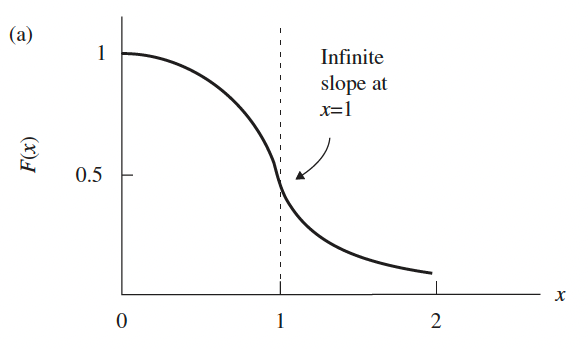
\includegraphics[scale=0.6]{images/F(x)jellium.png}
    \caption{Andamento di $F(x)$ con singolarità logaritmica in $x=1$}
    \label{fig:fxjellium}
\end{figure}
\newpage
\begin{figure}[!ht]
    \centering
    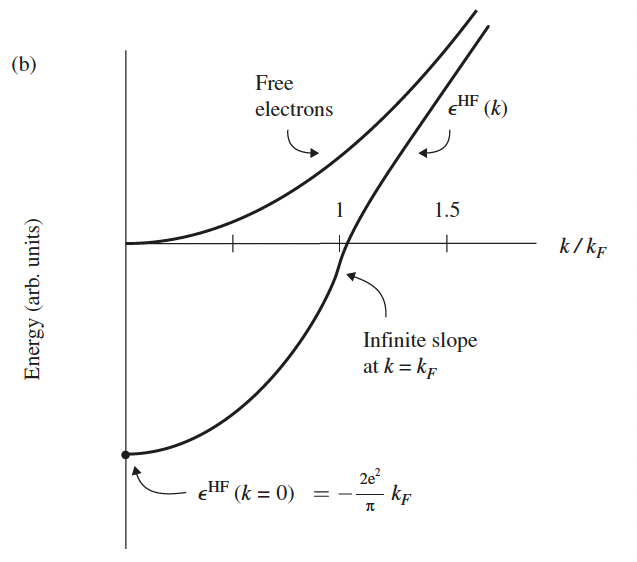
\includegraphics[scale=0.6]{images/energyjellium.png}
    \caption{Energia di Hartree-Fock per un gas di elettroni interagenti confrontata con l'energia di un gas di elettroni liberi}
    \label{fig:energyjellium}
\end{figure}
\begin{equation*}
    \varepsilon_{\text{HF}}(\overline k)=\frac{\hbar^2k^2}{2m}+E_{\text X}(k)
\end{equation*}
Osserviamo che la velocità della funzione d'onda è definita come:
\begin{equation*}
    \overline v = \frac{1}{\hbar}\partialderivative{\varepsilon(\overline k)}{\overline k}
\end{equation*}
Per via del fatto che nella definizione di $F(x)$ c'è un punto di flesso verticale, la velocità diverge a $k_F$ nel modello di \textbf{Hartree-Fock}, il che non è buono. La velocità della sfera di Fermi controlla i sistemi elettrici e non possiamo avere $v \rightarrow +\infty$. Quindi il \textbf{modello di Hartree-Fock} non si comporta molto bene in questo modello. Ciò che manca è l'\textbf{energia di correlazione}. (pagina 124 Grosso-Parravicini)

%%%%%%%%%%%%%%%%%%%%%%%
%%%%%% Lezione 5 %%%%%%
%%%%%%%%%%%%%%%%%%%%%%%

\lecture{5}{18/10/2021}
Per valutare l'energia totale di Hartree-Fock nello stato fondamentale possiamo sommare tutte le energie dei vari orbitali, tenendo conto della degenerazione di spin (fattore $2$) e dividendo per $2$ rimuovendo il doppio conteggio che appare nell'andare a valutare l'interazione elettrone-elettrone.
\begin{equation*}
    E= 2 \sum_{|\overline k|<k_F} \frac{\hbar^2k^2}{2m} + \sum_{|\overline k|<k_F}E_X(\overline k)
\end{equation*}
Il primo termine è l'energia cinetica per un sistema di particelle nella sfera di Fermi, che possiamo definire come:
\begin{equation*}
    N\expval{\varepsilon}=N\frac 35 \varepsilon_F
\end{equation*}
Se siamo interessati in particolar modo all'energia media per particella abbiamo:
\begin{equation*}
    \begin{aligned}
        \frac E N &= \frac 35\varepsilon_F+\frac 1N \sum_{|\overline k|<k_F}E_X(\overline k) \\
        & = \frac 35\varepsilon_F+\frac 1N V \int_{|\overline k|<k_F}\dd[3]{k}\frac{E_X(\overline k)}{(2\pi)^3}\\
        & = \frac 35\varepsilon_F+\frac 1\omega \frac{4\pi}{(2\pi)^3}\int_0^{k_F}\dd{k}k^2E_X(\overline k)\\
        & = \cdots \text{ Conti espliciti su Grosso Parravicini - Capitolo 4, Appendice C}\\
        & = \frac 35 \varepsilon_\text{F}- \frac 34\frac{e_0^2k_\text{F}}{\pi} \\
        & = \frac 35 \frac{\hbar^2k_\text{F}^2}{2m}- \frac 34\frac{e_0^2k_\text{F}}{\pi} \\
        & = \expval{\varepsilon_{\text{cinetica}}}+\expval{\varepsilon_{\text{X}}}
    \end{aligned}
\end{equation*}
Introduciamo l'\textbf{electron gas parameter} $r_\text S$ in relazione alla densità di elettroni:
\begin{equation*}
    \frac{4\pi}{3}(r_\text{S}a_0)^3=\frac 1 \omega
\end{equation*}
Tutte le energie possono essere espresse in \textit{Rydberg}: $\text{Ry}=\frac 12 \frac{e_0^2}{4\pi\varepsilon_0}\frac{1}{a_0}$, quindi:
\begin{equation*}
    k_\text{F}=(3\pi^2)^{\frac{1}{2}}\bigg(\frac{3}{4\pi}\bigg)\frac{1}{r_\text{S}a_0}
\end{equation*}
Inserendo questo risultato nell'energia media per particella abbiamo:
\begin{equation*}
    \varepsilon=\bigg(\frac{2.21}{r_\text{S}^2}-\frac{0.916}{r_\text{S}}\bigg)\text{Ry}
\end{equation*}
E descrive il caso \textbf{paramagnetico} di un gas di elettroni.
Per $r_\text{S}\rightarrow 0$, cioè nel limite di alta densità, l'energia cinetica domina sull'energia di interazione tra elettroni (basti guardare come scalano le densità) e il \textbf{modello di Hartree-Fock} descrive bene il comportamento di questi gas viceversa si comporta male nel limite di bassa densità.\\
Un'altra osservazione interessante che si può fare riguarda la definizione di $E_X$ in termini della funzione $F(x)$. Quest'ultima varia in modo smooth (da $1$ a $\frac 12$) non appena $k$ va da $0$ a $k_\text{F}$. Nel caso ipotetico in cui rimpiazziamo la funzione $F(x)$ con il suo valore medio $\frac 34$, avremo che il termine di scambio è costantemente uguale a:
\begin{equation*}
    E_\text{X}=-\frac32\frac{e_0^2}{\pi}k_{\text F}=-\frac32\frac{e_0^2}{\pi}(3\pi^2n)^{\frac 13}
\end{equation*}
Questo risultato può essere utilizzato per migliorare il \textbf{modello di Thomas-Fermi} per sistemi elettronici non omogenei di densità locale $n(\overline x)$:
\begin{equation*}
    E\big[n(\overline x)\big]=\int \dd[3]{x}V_{\text{ext}}(\overline x)n(\overline x)+E_\text{H}\big[n(\overline x)\big]+\int \dd[3]x n(\overline x)\frac 35\varepsilon_\text{F}(n(\overline x))+\int \dd[3]xn(\overline x)E_X(n(\overline x)) 
\end{equation*}
Questo modello è noto come \textbf{modello di Thomas-Fermi-Dirac}.\newline
Nell'approssimazione di Hartree-Fock, il normale stato fondamentale di un gas di elettroni è stato costruito da onde piane doppiamente occupate, di vettori d'onda confinati nella sfera di Fermi. Oltre al normale stato fondamentale, è interessante considerare la situazione estrema in cui tutti gli elettroni hanno spin parallelo. Vogliamo confrontare l'energia dello stato fondamentale della \textit{fase normale} (chiamata anche \textbf{fase paramagnetica}) con l'energia della \textit{fase completamente polarizzata} (detta anche \textbf{fase ferromagnetica}). Nel caso \textbf{paramagnetico}, occupiamo tutti i livelli fino a raggiungere l'\textbf{energia di Fermi}, nel caso \textbf{ferromagnetico}, necessitiamo di più livelli, più precisamente il doppio rispetto a quelli che avevamo nel paramagnetico. Pertanto se $k_\text{F}$ cambia, anche il volume diventa tanto maggiore:
\begin{equation*}
    2\frac{4\pi}{3}(k_{\text F}^{\text{p}})^3=\frac{4\pi}{3}(k_{\text F}^{\text f})^3
\end{equation*}
Abbiamo un fattore $2$ poiché tutti gli spin sono orientati lungo la stessa direzione e verso. Allora:
\begin{equation*}
    k_{\text F}^{\text f}=(2)^{\frac 13}k_{\text F}^{\text p}
\end{equation*}
E lo inseriamo nella relazione paramagnetica per ottenere il caso ferromagnetico:
\begin{equation*}
    \varepsilon^{\text f}=\bigg(\frac{2.21}{r_\text{S}^2}2^{\frac 23}-\frac{0.916}{r_\text{S}}2^{\frac 13}\bigg)\text{Ry}
\end{equation*}
Ci chiediamo a questo punto per quale valore della densità possiamo soddisfare la seguente disuguaglianza:
\begin{equation*}
    \varepsilon^{\text {ferrom.}} < \varepsilon^{\text {param.}}
\end{equation*}
Svolgendo i conti si ottiene che 
\begin{equation*}
    r_\text{S} > \frac{2\pi}{5}(2^{\frac 13}+1)\bigg(\frac{9\pi}{4}\bigg)^{\frac 13}=5.45
\end{equation*}
Abbiamo quindi una soluzione ferromagnetica per bassa densità quando $r_\text{S} > 5.45$. \\
Possiamo considerare le tipiche densità dei metalli, in particolare le tipiche densità di reticolo dei metalli (di conseguenza il numero di elettroni di valenza). Abbiamo che:
\begin{equation*}
    2<r_\text{S}<5.4
\end{equation*}
Osserviamo che il valore $5.45$ è minore del valore $r_\text{S}$ per il cesio (Cs): $5.62$. Ma il cesio che è un metallo alcalino, non è un metallo ferromagnetico, è un metallo paramagnetico. Il \textbf{modello di Hartree-Fock} non prevede il corretto comportamento e le proprietà magnetiche di un gas omogeneo di elettroni. Manca qualcosa, è un'altra falla nel \textbf{modello di Hartree-Fock}:
\begin{enumerate}
    \item Velocità di Fermi infinita (non corretto);
    \item Sbaglia la descrizione delle soluzioni magnetiche (caso del Cs).
\end{enumerate}
Ciò che manca nel \textbf{modello di Hartree-Fock} è l'\textbf{energia di correlazione}. L'energia del nostro sistema sarà quindi:
\begin{equation*}
    E=E_{\text{HF}}+E_{\text{CE}}
\end{equation*}
Se abbiamo un elettrone alla posizione $\overline x$ la probabilità di trovare un altro elettrone in $\overline{x}'$ dipende dalla distanza che separa questi due punti, in quanto tra loro è esercitata una forza repulsiva. La correlazione è intesa quindi sulla posizione occupata dagli altri elettroni. Come abbiamo detto questa correlazione non è presente nel modello di Hartree-Fock, perché la funzione d'onda di Hartree-Fock è un semplice prodotto di funzioni d'onda a singola particella. La probabilità di trovare un elettrone nella posizione $\overline{x}'$ non dipende dalla probabilità di trovare un elettrone nella posizione $\overline x$ se hanno spin opposto. Mentre elettroni con lo stesso spin dipendono l'uno dall'altro e la porbabilità congiunta di trovare in un punto spaziale, dipende dalla distribuzione spaziale degli altri elettroni per via del termine di scambio. È quindi una manifestazione delle forze di scambio.
Calcolare l'energia di correlazione è difficile, c'è un sistema che va oltre al modello di Hartree-Fock e proviene dalla \textbf{teoria delle perturbazioni} e richiede:
\begin{itemize}
    \item Nuovi metodi perché non possiamo fermarci al secondo ordine, vogliamo considerare un numero infinito di ordini;
    \item \textbf{Teoria delle perturbazioni a molti corpi};
    \item L'oggetto matematico: \textbf{funzione di Green a molti corpi}; 
    \item Analisi diamagnetica della teoria delle perturbazioni dei diagrammi di Feynman,
\end{itemize}
Questo risultato, siccome siamo in regime perturbativo, può essere ottenuto solo ad alte densità, cioè per piccoli valori di $r_\text{S}$. A ricavarlo furono Gell-Mann e Brueckner (1957):
\begin{equation*}
    \varepsilon=\bigg(\frac{2.21}{r_\text{S}}^2-\frac{0.961}{r_\text{S}}+\varepsilon_{\text C}(r_\text{S})\bigg)\text{Ry}
\end{equation*}
dove
\begin{equation*}
    \varepsilon_{\text C}(r_\text{S})=-0.096+0.0622\ln{\varepsilon_{\text C}(r_\text{S})}
\end{equation*}
Questo ricordiamo per $r_\text{S}<1$ ed è una soluzione analitica della teoria delle perturbazioni.
Recentemente (40 anni fa) è stato introdotto un metodo differente che è un approccio stocastico \textbf{simulazioni Monte-Carlo quantistiche} ancora più complicato del precedente, qui non abbiamo più soluzioni analitiche, ma numeriche. Il risultato proviene da un metodo di valutazione stocastica della funzione d'onda che ci permette di ottenere l'energia di correlazione. Ceperly e Alden (1980) sono stati capaci di stimare l'energia di correlazione per un gas di elettroni omogeneo come funzione della densità:
[GRAFICO DI CEPERLY VEDI PHYSICAL REVIEW LETTER]
Quello che si nota è che la transizione dal comportamento paramagnetico al comportamento ferromagnetico è si verifica a $r_\text{S}=80$. Ci sono varie parametrizzazioni che spiegano questo risultato ad esempio una è dovuta a Perduew-Zuerger:
\begin{equation*}
    \begin{aligned}
    \varepsilon_{\text C}(r_\text{S})& =(-0.048+0.0311 \ln r_\text{S}-0.0116r_\text{S}+0.002r_\text{S}\ln r_\text{S})\text{Hartree}\\
    & =2(-0.048+0.0311 \ln r_\text{S}-0.0116r_\text{S}+0.002r_\text{S}\ln r_\text{S})\text{Ry}
    \end{aligned}
\end{equation*}
I primi due termini non sono nient'altro che il risultato ottenuto da Gell-Mann e Brueckner. Ovviamente questo vale sempre per $r_\text{S}<1$, mentre per $r_\text{S}>1$ avremo:
\begin{equation*}
    \varepsilon_{\text C}(r_\text{S})=-\frac{0.1428}{1+1.0529\sqrt{r_\text{S}}+0.334r_\text{S}}
\end{equation*}
Per valori di $r_\text{S}$ molto grandi, entriamo in una nuova regione che prende il nome di \textbf{cristallo di Wigner} ($r_\text{S}=90$). Entrambe le soluzioni paramagnetiche e ferromagnetiche corrispondo a un gas omogeneo di elettroni. Se la densità diventa davvero piccola c'è un'altra configurazione che è molto favorevole e corrisponde a un cristallo di elettroni. Diventano localizzate su un reticolo cristallino, ma non sono a riposo, vibrano, oscillano attorno a un punto per mantenere la validità del principio di indeterminazione di Heisemberg. È una collezione di elettroni vibranti ed è possibile valutare l'energia di questi cristalli di Wigner vedendola come somma di due termini: 
\begin{itemize}
    \item Energia elettrostatica, interazione tra gli elettroni, elettroni e background e tra il background stesso;
    \item Energia dei fononi (vibrazioni degli elettroni attorno alla posizione di equilibrio).
\end{itemize}
Mostriamo i passaggi per ottenere l'energia totale, ovviamente non possiamo risolverlo analiticamente:
\begin{equation*}
    E_{\text{Coulomb}}=\frac 12 \int \dd[3]{x}\dd[3]{x'}n_{\text{tot}}(\overline x)n_{\text{tot}}(\overline{x}')\frac{e_0^2}{4\pi\varepsilon_0|\overline{x}-\overline{x}'|}
\end{equation*}
dove
\begin{equation*}
    n_{\text{tot}}=n_{\text{background}}-\underbrace{n(\overline x)}_{\mathclap{\text{Densità degli elettroni}}}
\end{equation*}
la densità degli elettroni è definita come:
\begin{equation*}
    n(\overline x)=\sum_{\overline n}\delta(\overline x-\overline n)
\end{equation*}
$\overline n$ non è nient'altro che il reticolo di Bravais degli elettroni. Dobbiamo quindi porre questa espressione della densità all'interno dell'integrale. Ma questa somma converge molto lentamente all'interno di questo integrale, c'è quindi un trucco per velocizzarne la convergenza e prende il nome di \textbf{Trasformazione di Ewald}: anziché considerare una funzione delta, consideriamo una funzione delta a cui togliamo una gaussiana e poi aggiungiamo una gaussiana:
\begin{equation*}
    \delta \rightarrow (\delta-G)+G
\end{equation*}
Il problema di questa lenta convergenza è dovuta al fatto che l'interazione coulombiana è a lungo raggio, dobbiamo andare molto lontani per far convergere questa quantità. Supponiamo di usare questo trucco e inserirlo nell'integrale: la prima gaussiana corrisponde a un sistema neutro perché globalmente la carica è nulla e dal momento che questa carica totale è nulla, converge molto velocemente nello spazio reale. La seconda gaussiana corrisponde a un'interazione di una carica reale e interagisce con tutte le cariche, ma questa carica non è una carica puntiforme che farebbe convergere molto lentamente, ma abbiamo una "brodered charge" che fa convergere velocemente la somma (ARTICOLO ELEARNING 2020-2021).
Se risolviamo l'integrale otteniamo l'energia di Coulomb che dipende dal tipo di reticolo e dai parametri del reticolo come la densità, dimensione,... In particolare otteniamo che il miglior reticolo che possiamo scegliere (più bassa energia) è il reticolo BCC: body centered cubic lattice:
[IMMAGINE DEL BCC]
\begin{equation*}
    \varepsilon=-\frac{1.79}{r_\text{S}}\text{Ry}
\end{equation*}
questa è quindi l'energia per elettrone, è un'energia classica (Hartree), ma non è zero. Nel jellium ricordiamo che questa energia era nulla, ma se localizziamo gli elettroni in un background uniforme, l'interazione di Coulomb non è più nulla.\\
Dal momento che non abbiamo particelle classiche, ma elettroni quantistici che vibrano attorno alla loro posizione di equilibrio, dobbiamo calcolare i fononi di questo reticolo bcc. Abbiamo una particella nella cella unitaria, abbiamo quindi una particella ad ogni lato del reticolo di Bravier e ci aspettiamo quindi tre relazioni di dispersione per i fononi (3 bande):
GRAFICO[OMEGA IN FUNZIONE DI Q]
In un cristallo, oltre alle modalità acustiche trasverse abbiamo una modalità acuistica longitudinale. Ma qui non abbiamo un cristallo vero come il cloruro di sodio. Nel cristallo di Wigner le cariche positive sono cristallizzate e questo ci dà un differente comportamento della modalità longitudinale che non è più acustica ma costante. Il valore di questa frequenza prende il nome di frequenza di plasma e dipende dalla densià:
\begin{equation*}
    \omega_p^2=\frac{e_0^2n}{\varepsilon_0m}
\end{equation*}
Con i fononi possiamo ottenere l'energia media dovuto al loro contributo:
\begin{equation*}
    \varepsilon_J(q)=\hbar\omega_J(q)(n_J(q)+\frac 12)
\end{equation*}
$J$ rappresenta l'indice di banda (branch index) mentre $n_J(q)$ è un intero che dipende dal grado di eccitazione di questi fononi. Se siamo a $T=0K$ abbiamo l'energia di punto zero:
\begin{equation*}
    E_{ZPE}=\sum_{Jq}\frac{\hbar\omega_j(q)}{2}
\end{equation*}
Se vogliamo l'energia di punto zero per particella:
\begin{equation*}
    \frac{E_{ZPE}}{N}=\frac 1N\sum_{Jq}\frac{\hbar\omega_j(q)}{2}=\frac 1N\sum_j\underbrace{V}_{\mathclap{\text{Zona di Brilloun}}}\int \frac{\dd[3{q}]}{(2\pi)^3}\frac{\hbar\omega_j(q)}{2}=\frac{1}{\omega}\sum_{J=1}^3\int \frac{\dd[3{q}]}{(2\pi)^3}\frac{\hbar\omega_j(q)}{2}
\end{equation*}
Risolvendo analiticamente otteniamo:
\begin{equation*}
    \varepsilon_{\text {WC}}=\bigg(\frac{2.66}{r_\text{S}^{\frac 32}}-\frac{1.79}{r_\text{S}}\bigg)\text{Ry}
\end{equation*}
Questo risultato rappresenta l'energia per particella in un cristallo di Wigner per valori di $r_\text{S}$ molto grandi.\\
Wigner propose prima della soluzione Monte Carlo quantistica una possibile forma dell'energia di correlazione che è in grado di interpolare i valori compresi tra i risultati di Gell-Mann Brucker e tra i valori dei cristalli di Wigner:
\begin{equation*}
    \varepsilon_\text{CE}^\text{Wigner}=-\frac{0.88}{7.8+r_\text{S}}\text{Ry}
\end{equation*}
Torniamo al caso dei metalli, cosa ci aspettiamo di vedere in un metallo reale? Abbiamo visto che il modello di Hartree-Fock non è più un buon modello per valutare l'enegia di coesione di un metallo, cioè l'energia che otteniamo nel formare un metallo. Ma anche se considerassimo l'energia di correlazione non è sufficiente perché nei metalli reali, abbiamo i nuclei ai lati del reticolo e non sono omogeneamente BRODERED. Supponiamo di considerare una correzione all'energia di Hartree dovuto al fatto che localizziamo l'energia dei nuclei. Nel jellium l'energia di Hartree è nulla. Supponiamo di rifinire un modello e considerare che gli elettroni sono ancora distribuiti in maniera omogenea, ma localizziamo la carica dei nuclei. Se facciamo questo l'energia di Hartree non è più nulla, ma sappiamo esattamente quanto è grande perché è la stessa calcolata per il cristallo di Wigner se consideriamo un reticolo BCC per i nuclei:
\begin{equation*}
    \varepsilon=\varepsilon_{\text{HF}}-\frac{1.79}{r_\text{S}}\text{Ry}=\bigg(\frac{2.21}{r_\text{S}^2}-\frac{0.416}{r_\text{S}}-\frac{1.79}{r_\text{S}}\bigg)\text{Ry}
\end{equation*}
Possiamo usare questa energia per valutare la densità di equilibrio del nostro sistema:
\begin{equation*}
    \derivative{\varepsilon}{r_\text{S}}=0 \Rightarrow r_\text{S} = 1.65
\end{equation*}
Questo valore ci dà la densità di equilibrio di un gas di elettroni. Questo valore sembra piccolo, perché i valori tipici di $r_\text{S}$ sono in un intervallo $2<r_\text{S}<5.6$. C'è qualcosa che manca, considerare la correlazione non è sufficiente per ottenere $r_\text{S}$ per i metalli reali. Possiamo migliorare questa soluzione senza andare a trattare gli elettroni di banda, ma considerando solo gli elettroni di valenza.